\chapter{Data collection of three simultaneous sensors}

The electrical resistance of the thin films was monitored in reaction to different volatile organic compounds (VOCs) at constant operating temperatures in order to conduct gas-sensing studies. Under dynamic flow conditions set by mass flow controllers with different capacities, the sample gases were infused. 
\begin{figure}
    \centering
    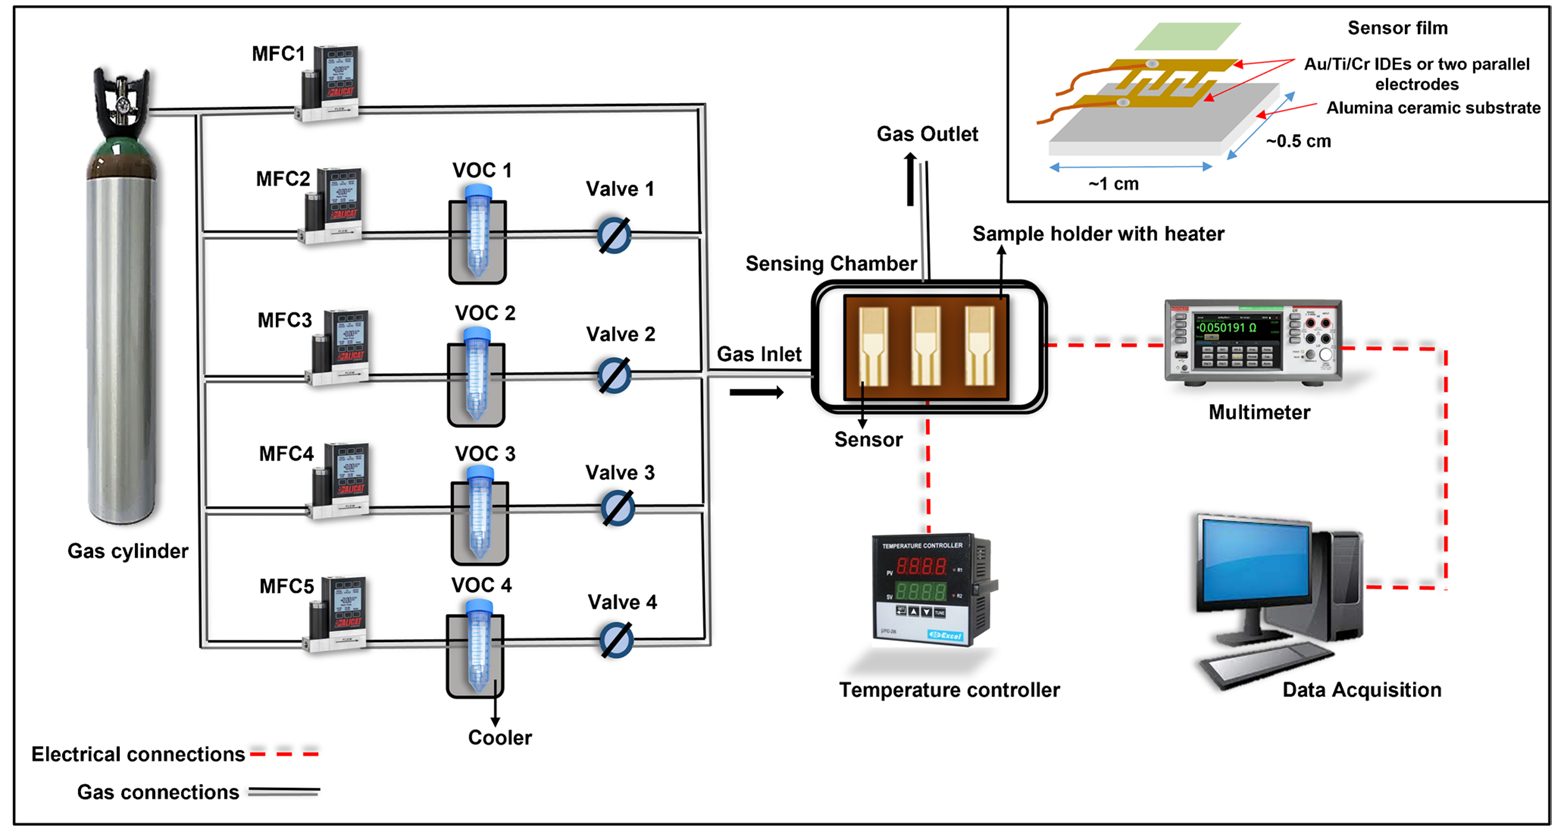
\includegraphics[width=1\linewidth]{Thesis Prashant//Images//Figures/gas sensing setup.png}
    \caption{ The schematic diagram of the gas sensing setup used for the experiment \cite{singh2024metal}}
    \label{fig:enter-label}
\end{figure}
The in-house gas sensing system employed in this study is shown in Figure 1. In order to assess the gas sensing characteristic in a detecting chamber, the films were placed on a sample holder that could achieve 400°C utilizing a heater underneath the sample holder (manufactured by Excel Instruments, India). The temperature of the sensor was determined using a sample holder with a type-K thermocouple installed. For measuring sensor resistance, an alumina substrate with interdigitated gold electrodes is used. The sensor resistance was measured using a Keithley 6517B electrometer connected to a workstation by providing two probes with a constant bias voltage of 10 V. With a tolerance of 1 fA, it is a high-resistance analyzer that could contribute meaningfully to  1015 ohms. To evaluate the sensor sensitivity to ethanol and other volatile organic compounds, the deposited films need to be exposed to the relevant vapours diluted in the air. \cite{singh2024metal}




